\subsection{Planning}
Le planning se présente sous la forme d'un diagramme de Gantt, montré ci dessous, qui nous permet de comparer le travail effectué et le travail prévu.
Ce Gantt est disponible en format global et en format détaillé sur le SharePoint CapProjet.
Un planning prévisionnel des tâches est également crée chaque semaines de travail.
Il est accessible dans le même document que le Gantt, dans les onglets.

\begin{figure}[h!]
	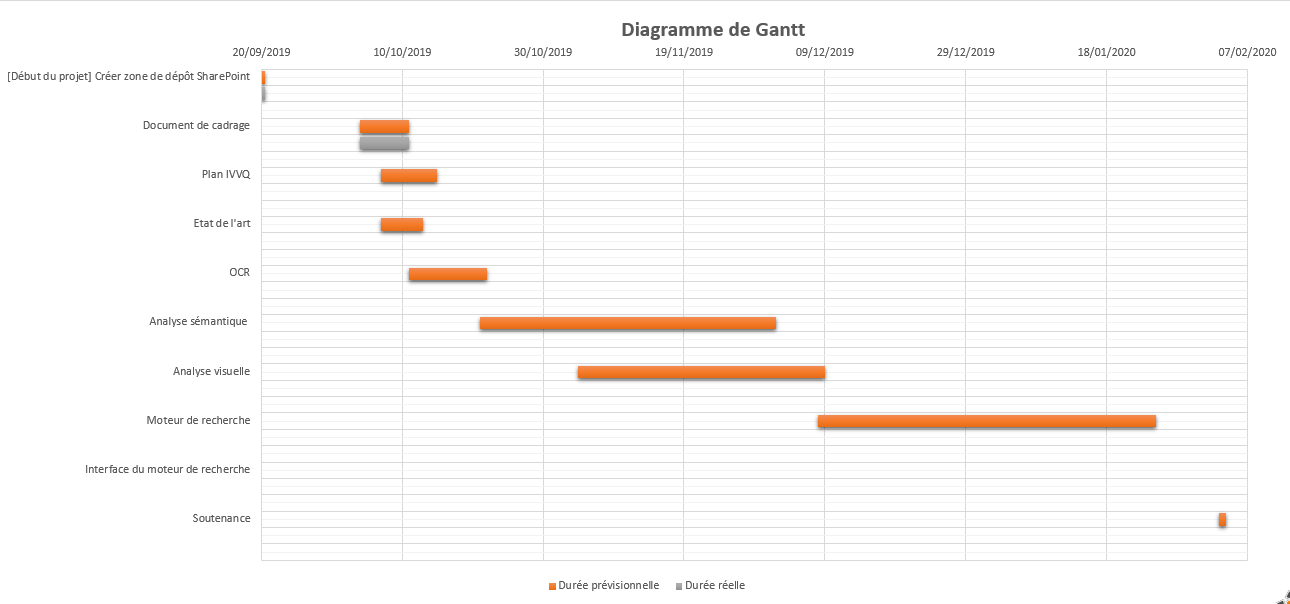
\includegraphics[width=\linewidth]{images/gantt.png}
	\caption{Gantt prévisionnel}
	\label{fig:MC}
\end{figure}		


\subsection{Gouvernance}
\subsubsection{Fonctionnement de l'équipe avec le mentor}
Notre première réunion avec notre mentor, Patricia Besset-Véziat, nous a permis de mettre au point nos règles de fonctionnement.
Nous avons convenu d'une réunion de suivi par semaine afin de vérifier l'avancement et la bonne conduite du projet.
Cette réunion n'est pas nécessairement en face à face et pourra être réalisée en visioconférence.


\subsubsection{Fonctionnement de l'équipe avec le commanditaire}
Nous avons convenu avec le commanditaire d'une méthode de travail agile.
Pour cela, nous envisageons une réunion de suivi toutes les deux semaines, et une réunion de pilotage tous les mois.
La réunion de suivi sera faite par visioconférence ou par échange de mails informatifs du travail réalisé et des éventuelles questions.
La réunion de pilotage sera réalisée en face à face, à l'ESIEA Laval ou à la Prefecture de Mayenne, chez le commanditaire.
Cette réunion a pour objectif de présenter l'avancement du projet et de discuter des éventuels changements désirés par le commanditaire, conformément à l'interaction client de la méthode agile.


\subsubsection{Fonctionnement interne de l'équipe}
Le fonctionnement interne du groupe est axé autour de la méthode agile.
Nous allons faire une réunion de planning une fois par semaine au début de la semaine afin de déterminer le programme de travail de la semaine à venir, et une réunion à la fin de la semaine pour faire le point sur les tâches effectuées.
Au cours de la semaine, nous resterons en communication le plus possible malgré la distance Paris/Laval qui limite les interactions directes.


